\section{模型评估和分析} % 罗哲焱

\subsection{数据集分析}

我们在给定的训练集和测试集上进行实验,训练集中的每条数据包含评论ID、评论内容与攻击性评分,测试集则只包含评论ID和评论内容。每句评论内容是由英文词组组成的句子。我们将攻击性评分大于等于0.5的评论视为攻击性评论,模型需要预测的是一句话具有攻击性的概率。表~\ref{tab:dataset}~展示了数据集的统计信息。可以看到攻击性的评论只占全部样本数的约8\%,是一个非常不平衡的数据集。

\begin{table}[htbp]
    \centering
    \begin{tabular}{ccccccc}
    \toprule
        & 样本数 & 最大单词个数 & 攻击性评论数 \\
        \midrule
        训练集 & 1777800 & 317 & 142178 \\
        测试集 & 27074 & 202 & - \\
        \bottomrule
    \end{tabular}
    \caption{数据集统计信息}
    \label{tab:dataset}
\end{table}

进一步地,我们对含有特定词汇的语句进行了统计,图~\ref{fig:toxic}~展示了包含不同词汇的攻击性评论个数。不同的评论背景下,攻击性评论占比不同,例如包含``black''的评论中有接近三分之一都含有攻击性,并且在这些背景下,有攻击性的比率都高于训练集中所有评论中恶意评论的比率8\%。

\begin{figure}[htbp]
    \centering
    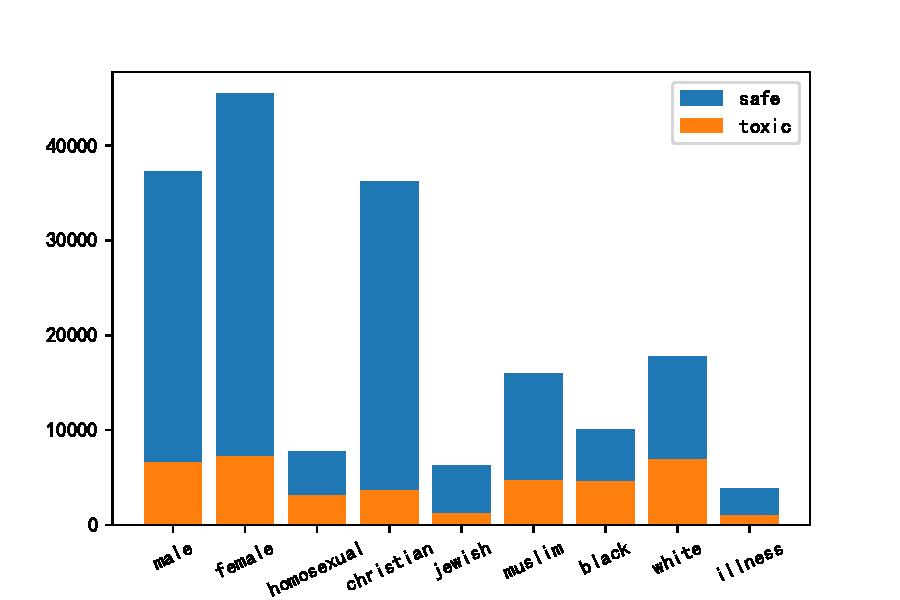
\includegraphics[width=.56\textwidth]{figs/toxic.pdf}
    \caption{不同背景下的攻击性评论数}
    \label{fig:toxic}
\end{figure}

\subsection{评价指标}

对于模型输出的概率,使用Bias AUC评判模型的好坏,Bias AUC是一个改进版的AUC指标,用于纠正可能存在的模型偏差,达到考察模型去偏能力的作用。

Bias AUC包含4项不同的AUC,每个AUC使用测试集不同的部分进行评价:

\begin{itemize}
    \item {\bf 全体AUC}:在所有数据上计算AUC。
    \item {\bf 子集AUC}:选取出包含特定词汇(如``male'', ``female''等)的评论计算AUC。
    \item {\bf BPSN AUC}:对于特定的词汇,在非恶意评论中选出带有这些词的评论,在恶意评论中选取\textbf{不}包含这些词汇的评论计算AUC。
    \item {\bf BNSP AUC}:对于特定的词汇,在非恶意评论中选出\textbf{不}带有这些词的评论,在恶意评论中选取包含这些词汇的评论计算AUC。
\end{itemize}

最终指标Bias AUC由这几项加权平均得到:

\begin{equation}
\begin{aligned}
     Bias\_AUC &= \frac{1}{4} Overall\_AUC + \frac{1}{4}(\frac{1}{|G|}\sum_{g\in G}Subgroup\_AUC_g^{-5})^{-\frac{1}{5}} \\
     &+ \frac{1}{4}(\frac{1}{|G|}\sum_{g\in G}BPSN\_AUC_g^{-5})^{-\frac{1}{5}} + \frac{1}{4}(\frac{1}{|G|}\sum_{g\in G}BNSP\_AUC_g^{-5})^{-\frac{1}{5}}
\end{aligned}
\end{equation}

\subsection{实现细节}

\subsubsection{基础方法}

将文本分词以后输入BERT模型,使用[CLS]标签的输出,通过线性分类器进行分类。设定学习率为$10^{-5}$,权重衰减为$10^{-5}$。使用Adam优化器进行优化。分类器特征随机丢弃(Dropout)的概率设为0.1。我们在全数据集上每300次更新进行一次测试,取验证集上表现最好的模型作为最终的模型,得到测试集上的预测结果。

\subsubsection{去偏方法}

综合考虑模型性能以及算力需求,在不变解释的框架中,分别使用三个参数不共享的DistilRoBERTa模型\cite{YinhanRoBERTa2019}作为生成器$g(\textbf{\textit{X}})$和检测器$f_i(\textbf{\textit{Z}}),f_e(\textbf{\textit{Z}},E)$的骨干模型。对于环境相关的检测器$f_e(\textbf{\textit{Z}},E)$,环境嵌入依次和该样本中所有单词嵌入相加,再输入到之后的骨干模型中。对于生成器$g(\textbf{\textit{X}})$得到的遮罩$m$,强制第一位为$1$,保证表征句子特征的特殊单词[CLS]在下游的检测器中。

由于train\_extra.json中类别的缺失较多,关于环境变量的生成,参考Chuang等人\cite{chuang2021mitigating}基于规则的工作,采用将基于规则和train\_extra.json标注相结合的方法构建。使用正则表达式,匹配句子中特定的单词出现,将句子分为``有不针对少数群体的恶意单词'',``有针对少数群体的恶意单词'',``有针对少数群体的单词(但无恶意)''和``其他''共四类。每一类的嵌入保证和单词嵌入维数相同,并使用随机初始化。

所有句子统一填充或截取到256个单词。

\subsection{超参数调优}

由于训练集过于庞大,而预训练模型训练过于耗时,每次利用全数据进行训练并进行参数调整会使得开销增大,因此我们先在基线模型上划分出不同量的训练数据进行测试,并利用少量数据对我们的模型调优。具体来说,TextCNN模型上不同数据量的表现如表~\ref{tab:textcnn}~所示,其中验证集通过从训练数据中划出5\%或10\%留出得到,在数据量较大时选择留出比例更小的验证集。最终,我们用$10^5$条数据进行训练并调优我们的模型,从中我们划出5\%作为验证集。在最终训练时使用全部的训练数据,使用2\%的数据进行验证。

\begin{table}[htbp]
    \centering
    \begin{tabular}{ccccccc}
        \toprule
        训练数据条数 & 验证集Bias AUC & 测试集Bias AUC \\
        \midrule
        $10^5$ & 89.22 & 88.83 \\
        $5\times 10^5$ & 90.10 & 89.94 \\
        $1.78\times 10^6$ & 91.29 & 91.32 \\
        \bottomrule
    \end{tabular}
    \caption{不同量训练数据下TextCNN的表现}
    \label{tab:textcnn}
\end{table}

\subsection{结果对比}

经过模型训练和超参数调整,我们对比了不同方法的效果,结果如表~\ref{tab:results}~所示,评测指标采用Bias AUC。最终我们发现经过微调后的预训练BERT模型取得了最优的效果,而加入不变解释框架的去偏算法的性能不太理想,在测试集的准确率降低了2个百分点。可能的原因是敏感身份词的标注缺失值较多,模型无法很好地消除环境因素。最终我们的模型在比赛工作站上取得了第6名的成绩,如图~\ref{fig:rank}~所示。

\begin{table}[htbp]
    \centering
    \begin{tabular}{lc}
        \toprule
        \multicolumn{1}{c}{模型} & Bias AUC \\
        \midrule
        TextCNN & 91.32 \\
        AdvBERT & 92.96 \\
        InvRat & 91.20 \\
        DistilBERT & 92.08 \\
        BERT & {\bf 93.41} \\
        \bottomrule
    \end{tabular}
    \caption{模型表现对比}
    \label{tab:results}
\end{table}

\begin{figure}[htbp]
    \centering
    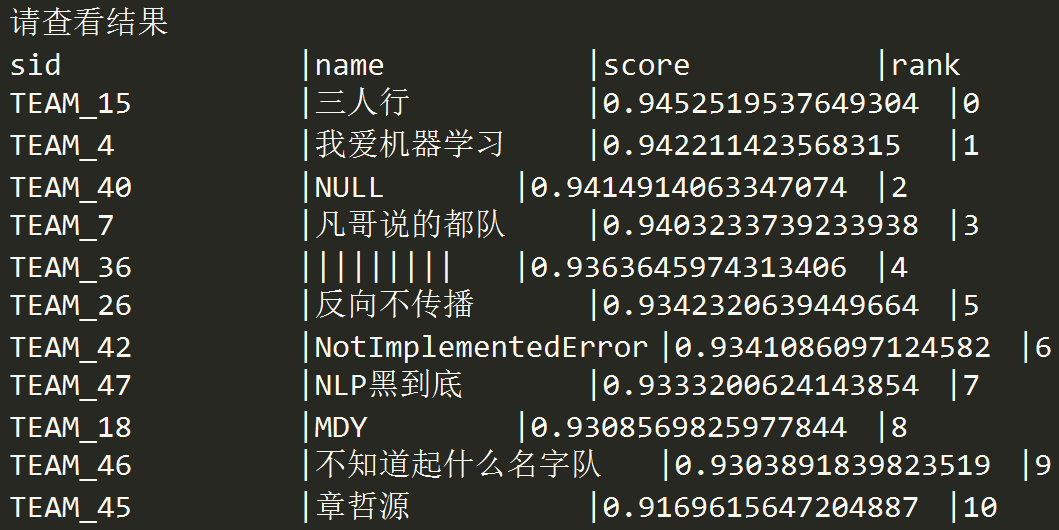
\includegraphics[width=.8\textwidth]{figs/rank.png}
    \caption{比赛工作站排名截图}
    \label{fig:rank}
\end{figure}
